\documentclass[a4paper,11pt]{article}

\usepackage[margin=3cm]{geometry}

\usepackage{graphicx}
\usepackage{subcaption}
\usepackage[colorlinks,allcolors=violet]{hyperref}
\usepackage{url}
\usepackage[dutch]{babel}

% https://tex.stackexchange.com/questions/94032/fancy-tables-in-latex
\usepackage[table]{xcolor}
\usepackage{booktabs}

\usepackage[utf8]{inputenc}

% https://tex.stackexchange.com/questions/664/why-should-i-use-usepackaget1fontenc
\usepackage[T1]{fontenc}
\usepackage{microtype} % good font tricks

\newcommand{\note}[1]{{\colorbox{yellow!40!white}{#1}}}
\newcommand{\exampletext}[1]{{\color{blue!60!black}#1}}

\begin{document}

\noindent
\colorbox[HTML]{52BDEC}{\bfseries\parbox{\textwidth}{\centering\large
  --- Report P\&O CW 2019--2020 Task ST2.1 ---
}}
\\[-1mm]
\colorbox[HTML]{00407A}{\bfseries\color{white}\parbox{\textwidth}{
  Department of Computer Science -- KU Leuven
  \hfill
  \today
}}
\\

\smallskip

\noindent
%\mbox{}\hfill
\begin{tabular}{*4l}
\toprule
\multicolumn{2}{l}{\large\textbf{Team 12}} \\
\midrule
Martijn Debeuf &  10000h\\ % fill in the time spend on this task per team member who worked on it
Toon Sauvillers &  10000h\\
Seppe Van Steenbergen & 10000h \\
\bottomrule
\hline
\end{tabular}\\
\\

\noindent
{\color[HTML]{52BDEC} \rule{\linewidth}{1mm} }

\section{Introductie}\label{sec:introductie}
	Het herkennen van schermen, deze identificeren, lokaliseren uit een foto. Dit verslag behandeld deze uitdagingen. Het zoeken van schermen begint bij een foto. Deze foto bevat een scherm met een bepaald uitzicht, er is gekozen voor een groen-blauwe rand waarop gefilterd kan worden. Vervolgens zoekt het algoritme in de gefilterde foto naar aparte schermen en geeft aan hen een id. Met behulp van het kleurenverschil en bepaalde hoeken wordt de oriëntatie bepaald.

Het identificeren van het scherm gebeurd op dit moment nog apart met een kleurenbarcode. Deze barcode bevat 5 verschillende kleuren waardoor er 120 verschillende schermen geïdentificeerd kunnen worden. In de volgende weken worden deze twee, lokaliseren en identificeren, bij elkaar gezet.
\\
Dit verslag behandeld de keuzes die gemaakt zijn alsook een uitleg bij de gebruikte algoritmen en hun tijdscomplexiteit. De mogelijke beperkingen worden met deze kennis geduid.

\section{Methode}\label{sec:methode}
	Verschillende componenten zijn nodig om kleuren te vergelijken. Als eerste wordt de kleur bijgehouden die op de foto staat. Daarnaast is ook de herkende kleur belangrijk. Zowel voor HSL als voor RGB kijkt het algoritme naar de kleurafstand. Bij RGB is dit de Euclidische kleurafstand. 
$$ \mid RGB \mid = \sqrt{(R_1 - R_2)^2 + (G_1 - G_2)^2 + (B_1 - B_2)^2}$$
De methode vergelijkt zo elke pixel met de ``{\it perfecte}'', te detecteren kleuren. De gedetecteerde kleur zal deze zijn met kleinste afstand tot de pixel. Op dezelfde manier zal ook HSL werken. Deze zal echter enkel kijken naar de hue-waarde, voor zwart en wit kijkt het algoritme naar de lichtheid. In tabel \ref{tab:kleuren}  staan de genomen waarden van de ``{\it perfecte}'' kleuren.

\begin{center}
\begin{table}
\label{tab:kleuren}
\centering
\begin{tabular}{ | l | c | c | }
\hline
Kleur & [R, G, B] & Hue \\
\hline
Rood & [255, 0, 0] & 0 en 360 \\
Groen & [0, 255, 0] & 120 \\
Blauw & [0, 0, 255] & 240 \\
Geel & [128, 128, 0] & 60 \\
Cyaan & [0, 128, 128] & 180 \\
Magenta & [128, 0, 128] & 300 \\
Wit & [255, 255, 255] & $L <= 10$ \\
Zwart & [0, 0, 0]] & $L >= 90$ \\
\hline
\end{tabular}
\caption{De RGB en hue waarden van de ``{\it perfecte}'' kleuren.}
\end{table}
\end{center}

Een database houdt de waarden van alle getrokken foto's bij. Het onderzoek gebruikt de verschillende eigenschappen van deze foto's. De bijgehouden eigenschappen zijn: gedetecteerde kleur, dekking van de gedetecteerde kleur, alsook de dekking van de verwachte kleur, afstand van de perfecte tot de gedetecteerde kleur, grootte van omgeving rond het scherm, soort lichtinval en de helderheid van het getrokken scherm.

\section{Achtergrond}\label{sec:achtergrond}
	Er bestaat natuurlijk een breed gamma aan fotofilters. De benodigde code voor dit onderzoek is geschreven in Python. Daarom is gekozen om vier filters uit de bibliotheek van OpenCV te gebruiken (zie sectie \ref{sec:methode}).  Een eerste toegepaste filter is de \textit{Gaussian Blur}, gevolgd door \textit{Median Blur} en \textit{Mean Blur}. Deze methodes kijken naar de pixels rond een centrale pixel om zijn kleurwaarde te bepalen. Ten slotte is er ook een minder gekende ontruismethode gebruikt namelijk de \textit{Fast Non-Local Mean Denoising}. Deze werkt anders dan de eerste drie, zie sectie \ref{subsec:fnlmd}.

\subsection{Methodes met kernelgrootte}
De volgende methodes maken gebruik van een kernelgrootte, concreet betekend dit dat het algoritme gaat kijken naar een aantal rondomliggende pixels om de nieuwe kleurwaarde te bepalen. Bij een kernelgrootte van drie zal er een vierkant met zijde drie rond de pixel getrokken worden. Elk algoritme gaat deze pixels anders interpreteren om een nieuwe waarde toe te kennen.
\subsubsection{Gaussian Blur}
De {\it Gaussian Blur} gaat kijken naar de omliggende pixels. Degenen die verder liggen, zullen minder invloed hebben dan degenen die dichterbij liggen. Een pure {\it Gaussian Blur} zou naar alle omliggende pixels kijken, ze gaan namelijk allemaal een bijdrage leveren. Door de zware berekeningen die hiermee gepaard gaan, kijkt deze blur enkel naar de omliggende pixels binnenin de door de kernelgrootte gedefinieerde omgeving. \cite{gaussianBlur}

\subsubsection{Median Blur}
Binnen de kern sorteert dit algortime de pixels van klein naar groot, vervolgens wordt de middelste waarde (mediaan) geselecteerd. De kleur van de centrale pixel van de kernel wordt dan op deze waarde geplaatst.

\subsubsection{Mean Blur}
Hier gebeurt hetzelfde als bij de {\it Median Blur} enkel neemt het algoritme hier het gemiddelde in plaats van de mediaan.

\subsection{Fast Non-Local Mean Denoising}
\label{subsec:fnlmd}
Aan  de hand van de kern worden binnen de afbeelding gelijkende kernels gezocht. Gelijkende kernen worden bij elkaar geplaatst. Van elk van deze groepen wordt dan het gemiddelde bepaald. Daarna wordt elke pixel in elke kern binnen die groep op de gemiddelde waarde geplaatst. \cite{fastExplanation}

\section{Bevindingen}\label{sec:bevindingen}
	In dit deel bekijkt het verslag of het al dan niet interessant is om de afbeeldingen te filteren. De eerste belangrijke indicator was tijdsconsumptie. Ook de filters onderling zijn vergelijkbaar met betrekking tot de herkenning van de kleur. Vervolgens kan gekeken worden of de kern grootte een invloed heeft op de resultaten. Ten slotte gaat het verslag na of filteren effectief het detecteren van de kleur positief beïnvloed. 

	\subsection{Kleurruimte}\label{subsec:kleurruimte}
		Detectie van kleuren kan binnen verschillende kleurruimten, in dit onderzoek zijn RGB en HSL gebruikt om de schakeringen te detecteren, in sectie \ref{sec:achtergrond} staat meer achtergrondinformatie hieromtrent. Een eerste bemerking in het verschil tussen RGB en HSL is dat HSL een betere detectieratio heeft voor alle kleuren, zie figuur \ref{fig:HSLvsRGB}. RGB herkent dan weer duidelijk beter het wit en het zwart. Dit verschil is toe te wijzen aan de restrictie op het herkennen van zwart en wit in HSL. De lichtsterkte moet ofwel kleiner dan 10 ofwel groter dan 90 zijn om respectievelijk zwart en wit te detecteren. Het is een strikte restrictie om beiden te herkennen.

Met uitzondering tot geel en cyaan zijn alle kleuren met een verschil van minstens 10\% beter herkend door HSL. Bij zowel groen, blauw, magenta als rood is HSL opmerkelijk beter. Deze kleuren gaan over, of leunen aan bij, 90\% detectieratio. De detectie van rood leunt zelfs aan tegen de 100\%.
Om kleuren te herkennen heeft HSL duidelijk een meerwaarde. Wit en zwart herkennen gebeurt best niet met een kleurdetectie, ze zijn vaak geïdentificeerd als een andere kleur, zie sectie \ref{subsec:kleuren} omtrent kleuren. Het contrast tussen deze twee is een betere keuze om ze te onderscheiden van elkaar.

\begin{figure}
	\center
	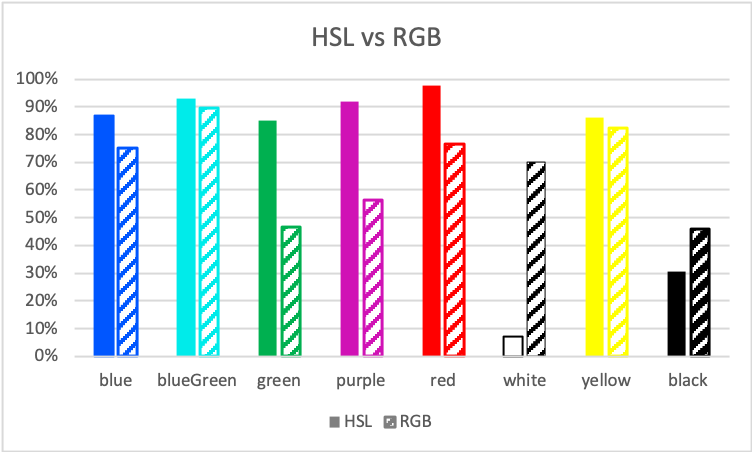
\includegraphics{img/HSLvsRGB}
	\caption{Verschil tussen juist gedetecteerde kleuren in HSL en RGB per kleur.}
	\label{fig:HSLvsRGB}
\end{figure}

				
	\subsection{Herkenning}\label{subsec:herkenning}
		\input{herkenning}
	\subsection{Omgevingsfactoren}\label{subsec:omgevingsfactoren}
		Dit verslag kijkt ook naar of verschillende omgevingsfactoren een effect hebben op het herkennen van kleuren. Zo zou de grootte van de omgeving de herkenning kunnen verbeteren of verslechteren, meer omgeving betekent namelijk dat de camera meer omgevingslicht binnenkrijgt. Alsook het licht kan een beïnvloedende factor zijn, de foto's behandelen twee soorten lichtinval: geen en artificieel licht. Buitenlicht zal niet besproken worden, de {\it Screen Caster} gaat ervan uit dat de schermen binnenshuis staan. Laatste omgevingsfactor is de helderheid van het scherm zelf. Heeft dit een grote invloed op de detectie? En hebben verschillende factoren een invloed op elkaar?

\subsubsection{Omgeving}
De foto's hebben verschillende groottes van omgeving. De omgeving kan groot ($\approx 80\%$), gemiddeld ($\approx 40\%$), klein ($\approx 10\%$) of niet aanwezig zijn. In figuur \ref{fig:omgeving}(a) zijn de bevindingen weergegeven. Per grootte van omgeving staat er weergegeven hoeveel procent van elke kleur juist werd gedetecteerd.

De detectie van kleuren gebeurd het beste bij een gemiddelde of kleine omgevingsgrootte. Wanneer de omgeving groot is, scoort de herkenning het slechtst. In figuur \ref{fig:omgeving}(b) staat per kleur welke kleur foutief is herkent, enkel en alleen bij een grote omgeving. Wat opvalt is dat vooral zwart als foute kleur naar voor komt en dan vooral bij groen, wit en geel. Dit is toe te wijzen aan het feit dat met meer lichtinval de schermen donkerder tonen op de foto. Door een grotere omgeving zal de artificiële inteligentie in de camera de focus niet meer op het scherm leggen. Als zwart niet meer nodig is en de restrictie op de lichtheid bij HSL niet meer geldt, kan dit probleem opgelost zijn, dit vergt echter verder onderzoek.
\begin{figure}
	\begin{subfigure}{0.5\textwidth}
	\centering
	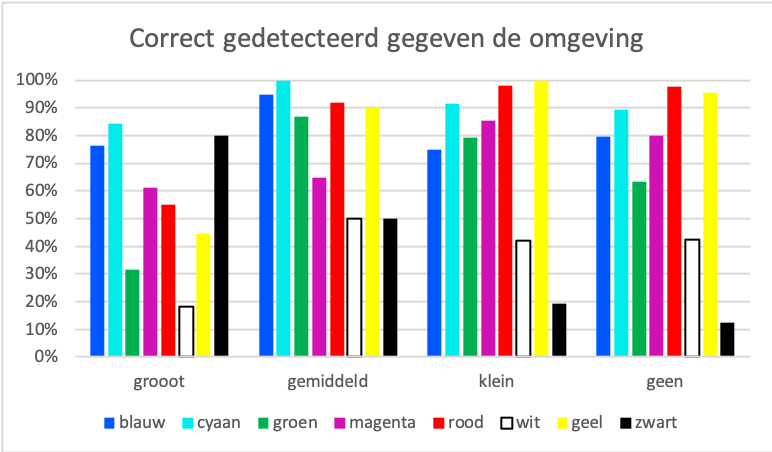
\includegraphics[scale=0.6]{img/Environment}
	\caption{Per kleur correct gedetecteerd met gegeven omgevingsgrootte.}
	\end{subfigure}
	\begin{subfigure}{0.5\textwidth}
	\centering
	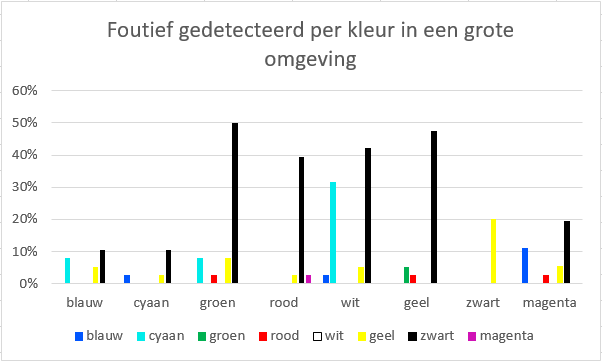
\includegraphics[scale=0.6]{img/BigEnvPerColor}
	\caption{Per kleur de foutief herkende kleur in grote omgeving.}
	\end{subfigure}
	\caption{Grafieken met betrekking tot de omgevingsgrootte.}
	\label{fig:omgeving}
\end{figure}

\subsubsection{Lichtinval}
Dit verslag behandelt twee soorten lichtinval, artificieel en helemaal geen lichtinval. In figuren \ref{fig:lichtinval}(a) en \ref{fig:lichtinval}(b) staan de gedetecteerde kleuren per kleur bij respectievelijk artificieel en geen lichtinval. Rood komt bij artificieel licht in elke kleur voor, dit is toe te wijzen aan het licht dat een rode schijn achterlaat op de schermen. Zonder achtergrondverlichting  komt vooral zwart terug foutief terug. Dit is te wijten aan het algoritme dat naast het scherm gedetecteerd heeft.

Zwart detecteren is opvallend slecht bij artificieel licht, door de strenge herkenning ($L < 10$) en reflectie is deze niet herkent bij artificieel licht. Geel en cyaan komen veel voor bij detectie van wit, ook hier is de strenge herkenning ($L > 90$) de oorzaak.

\begin{figure}
	\begin{subfigure}{0.5\textwidth}
	\centering
	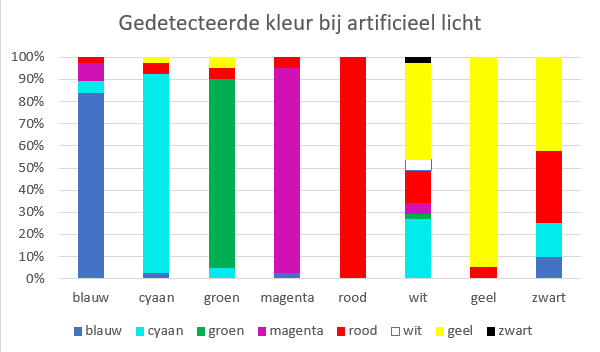
\includegraphics[scale=0.6]{img/artificialLightning}
	\caption{Artificieel lichtinval.}
	\end{subfigure}
	\begin{subfigure}{0.5\textwidth}
	\centering
	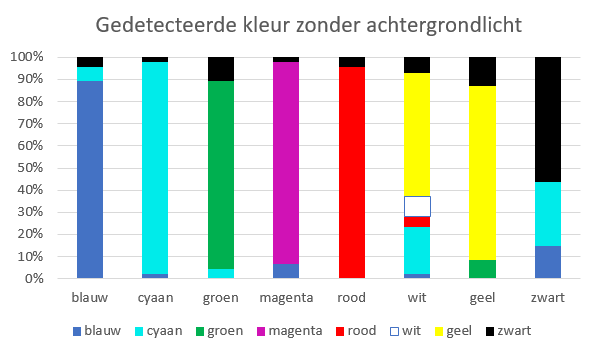
\includegraphics[scale=0.6]{img/noneLightning}
	\caption{Zonder lichtinval.}
	\end{subfigure}
	\caption{Gedetecteerde kleur per kleur. (HSL)}
	\label{fig:lichtinval}
\end{figure}

\subsubsection{Helderheid scherm}
In figuur \ref{fig:helderheid} staat het aantal procent correct gedetecteerde kleur per helderheid van het scherm. De laagste helderheid scoort het slechts, kleuren zijn donkerder en minder goed zichtbaar. Bij de drie andere helderheden is geen groot verschil op te merken. De schermhelderheid heeft geen grote invloed op de detectie van de schermen.
\begin{figure}
	\centering
	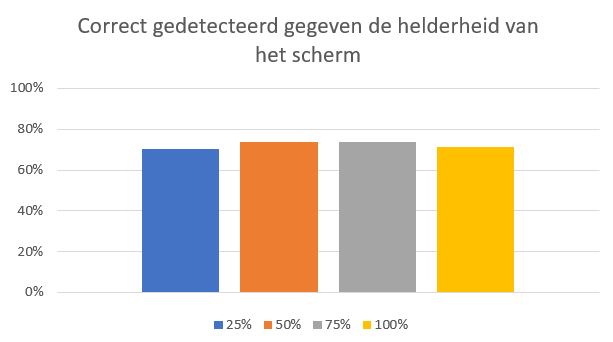
\includegraphics[scale=0.7]{img/brightness}
	\caption{Procent juist gedetecteerde kleur per kleur met gegeven schermhelderheid. (HSL)}
	\label{fig:helderheid}
\end{figure}


\section{Besluit}\label{sec:besluit}
	 
Uit de bevindingen is gebleken dat de interpretatie van kleur sterk afhankelijk is van de manier waarop kleur wordt voorgesteld en de omgevingsfactoren die hierbij aanwezig zijn. Enerzijds speelt de kleurruimte waarin een kleur wordt voorgesteld een grote rol bij de detectie. Van de verschillende kleurruimten die bekeken zijn, is er niet een die eenduidig beter is dan de andere. Beiden hebben hun voordelen, zo is HSL beter voor de detectie van alle kleuren dan RGB. Maar de detectieratio van zwart en wit is dan wel weer aannoemelijk beter in RGB dan in HSL.  Anderzijds spelen omgevingsfactoren ook een belangrijke rol bij de detectie van de kleuren. Hiervoor werd gekeken naar zowel de omgeving, de lichtinval en de helderheid van het scherm. De belangrijkste bevindingen hierbij hebben te maken met de lichtinval en de omgeving. Door lichtinval komt er bij artificieel licht extra rood in de kleuren door de rode schijn die het licht achterlaat. Hoe groter de omgeving, hoe meer de kleuren fout gedetecteerd gaan worden. Dit is te wijten aan het feit dat de camera hierbij op de omgeving gaat focussen in plaats van op het scherm. Tot slot is ook gebleken dat helderheid geen groot effect heeft op de detectie.
	
	\subsection{Toepassingen op het project}\label{subsec:toepassingen}
		Voor het detectiealgoritme kan het best gebruik gemaakt worden van de HSL kleurruimte zoals nu al het geval is. Maar voor het identificatiealgoritme waarbij wit en zwart gebruikt wordt, zou beter overgeschakeld worden naar een algoritme dat gebruik maakt van de RGB kleurruimte.

De keuze voor de drie kleuren die weergegeven worden op het detectiescherm valt op rood, groen en blauw. Deze drie kleuren hebben een grote detectieratio en de omgevingsfactoren hebben het minste invloed op deze kleuren.

Aan de hand van de bevindingen rondom omgeving moeten foto's zo dicht mogelijk getrokken worden bij de opstelling zodat de omgeving minimaal is. Natuurlijk moet wel heel de opstelling in de foto passen.




\end{document}